% ------------ LSA-proceedings-template.tex  -- LSA proceedings template ----------------------------------------------
% created by Sarah E. Murray, 24 April 2017 based on the LSA's stylesheet
% http://journals.linguisticsociety.org/proceedings/index.php/PLSA/pages/view/instructions
%Revised by Patrick Farrell, February 1, 2019 and March 8, 2020. 
%
% ------------ begin preamble -----------------------------------------------------------------------------------------
 \documentclass[12pt,letterpaper]{article}	
% ------------ personal packages ----------------------------------------------------------------------------
\usepackage{linguex}	%http://texdoc.net/texmf-dist/doc/latex/linguex/linguex-doc.pdf
% ------------ LSA page layout and packages ----------------------------------------------------------------------------
\usepackage{times}
\usepackage{natbib}
 	\setcitestyle{semicolon,aysep={},yysep={,},notesep={; }}
\usepackage{lipsum} % this and the following package and the settings beneath them are for maintaining indentation and still having ragged-right alignment
\usepackage{ragged2e}
\setlength\RaggedRightParindent{0.3in}
\RaggedRight

\usepackage{scrextend}  % this package and the following settings are for the footnote formatting
\deffootnote[.5em]{0em}{1em}{\textsuperscript{\thefootnotemark}\,}

\newcounter{savefootnote}   % these settings allow the use of an asterisk as a footnote label (for the author line below the title.
\newcounter{symfootnote}
\newcommand{\symfootnote}[1]{%
   \setcounter{savefootnote}{\value{footnote}}%
   \setcounter{footnote}{\value{symfootnote}}%
   \ifnum\value{footnote}>8\setcounter{footnote}{0}\fi%
   \let\oldthefootnote=\thefootnote%
   \renewcommand{\thefootnote}{\fnsymbol{footnote}}%
   \footnote{#1}%
   \let\thefootnote=\oldthefootnote%
   \setcounter{symfootnote}{\value{footnote}}%
   \setcounter{footnote}{\value{savefootnote}}%
}

\usepackage[labelsep=period]{caption}

\usepackage[margin=1.0in]{geometry}
\usepackage[compact]{titlesec}
	\titleformat{\section}[runin]{\normalfont\bfseries}{\thesection.}{.5em}{}[.]
	\titleformat{\subsection}[runin]{\normalfont\scshape}{\thesubsection.}{.5em}{}[.]
	\titleformat{\subsubsection}[runin]{\normalfont\scshape}{\thesubsubsection.}{.5em}{}[.]
\usepackage[usenames,dvipsnames]{color}	
\usepackage[colorlinks,allcolors={black},urlcolor={blue}]{hyperref} 		%likes to be last package 


% -------------- personal definitions ----------------------------------------------------------------------------
\usepackage{graphicx}  
\usepackage{subcaption}
\usepackage{color}
\usepackage[export]{adjustbox}

\definecolor{Red}{RGB}{255,0,0}
\newcommand{\red}[1]{\textcolor{Red}{#1}}
\newcommand{\jd}[1]{\textcolor{Red}{[jd: #1]}}
\definecolor{Blue}{RGB}{0,100,255}
\newcommand{\blue}[1]{\textcolor{Blue}{#1}}
\newcommand{\lk}[1]{\textcolor{Blue}{[lk: #1]}}

\newcommand{\citeA}{\textbf}

% -------------- LSA definitions ---------------------------------------------------------------------------------

%-------------------------------------------------------------- format abstract environment ------------------------
% Abstracts have to be 12pt, indented 1.4 inches on each side, and inline with the label
\renewenvironment{abstract}{%
\noindent\begin{minipage}{1\textwidth}
\setlength{\leftskip}{0.4in}
\setlength{\rightskip}{0.4in}
\textbf{Abstract.}}
{\end{minipage}}
%-------------------------------------------------------------- format keywords environment ----------------------
% Abstracts have to be 12pt, indented 1.4 inches on each side, and inline with the 
\newenvironment{keywords}{%
\vspace{.5em}
\noindent\begin{minipage}{1\textwidth}
\setlength{\leftskip}{0.4in}
\setlength{\rightskip}{0.4in}
\textbf{Keywords.}}
{\end{minipage}}

% ------------ end preamble -----------------------------------------------------------------------------------
% 
%
%
% ------------ begin main document ---------------------------------------------------------------------------
 
\begin{document} 

%%If using linguex, need the following commands to get correct LSA style spacing
%% these have to be after  \begin{document}
\setlength{\Extopsep}{6pt}
\setlength{\Exlabelsep}{9pt}		%effect of 0.4in indent from left text edge
%%
 
\begin{center}			%title and author lines
\normalfont\bfseries
Perceptual Difficulty Differences Predict Asymmetry in Overmodification with Color and Material Adjectives
\vskip .5em
\normalfont
{Leyla Kursat \& Judith Degen\symfootnote{Authors: Leyla Kursat, Stanford University (\href{mailto:lkursat@stanford.edu}{lkursat@stanford.edu}) \& Judith Degen, Stanford University (\href{mailto:jdegen@stanford.edu}{jdegen@stanford.edu}).}}
\vskip .5em
\end{center}

\begin{abstract}
When referring to objects, speakers are often more specific than they need to be for establishing unique reference. Adjectival overspecification patterns are not random, but structured: color adjectives are produced redundantly more often than size or material adjectives; color adjectives are more likely to be produced redundantly with increasing scene variation; and adjectives are more likely to be produced redundantly, the more atypical the property denoted by the adjective is for the object under discussion. The only current computational model of referring expression production that accounts jointly for all of these patterns is couched within the Rational Speech Act framework and assumes that adjectives differ in how noisy, and consequently, how useful they are for the purpose of establishing reference. One hypothesis about the nature of this noise is that it reflects the perceptual difficulty of establishing whether the property denoted by the adjective holds of the contextually relevant objects. Here, we take a first step towards testing the prediction that systematic differences in the overmodification patterns observed for color and material adjectives can be explained by a difference in perceptual difficulty of establishing whether objects are of a particular color or material. In Exp.1, we norm the perceptual difficulty associated with establishing whether an object exhibits a color or material and select objects with highest and lowest perceptual difficulty for testing in Exp. 2. In Exp. 2, we test in a reference game whether adjectives that denote more perceptually difficult properties indeed are less frequently produced redundantly. Finally in Exp. 3 we test the effect of perceptual difficulty beyond property type. 
\end{abstract}

\begin{keywords} %separated by semicolons
reference; perception; overinformativeness; experimental pragmatics
\end{keywords}

\section{Introduction} 

When referring to objects, speakers aim to be sufficiently informative in choosing which features of the object to include in their utterances. However, they are often more specific than they need to be for establishing unique reference. Recent research has identified systematic differences in adjectival overspecification patterns, but the question remains open why such patterns emerge.

One way in which we observe structure in the production of overinformative referring expression is through the asymmetry in the redundant use of color, size and material adjectives. When size or material is the sufficient property to single out the intended reference, participants routinely include color adjectives in their utterances. However, in contexts where color is sufficient for unique reference, speaker's don't tend to mention size or material redundantly (\citealt{Pechmann1989, Sedivy2003, GattEtAl2011, RubioFernandez2016, DegenEtAl2020}). Moreover, speaker's knowledge of the typicality of the properties of objects and the features of the context interact with these asymmetries. Color adjectives are more likely to be produced redundantly with increasing scene variation (\citealt{DegenEtAl2020, DaviesKatsos2013, KoolenEtAl2013}) and adjectives are more likely the be produced redundantly, the more atypical the property denoted by the adjective is for the object under discussion (\citealt{DegenEtAl2020, WesterbeekEtAl2015, Mitchell2013}).

Many explanations are offered in the literature for the source of overinformative referring expressions including pragmatic, semantic, lexical and visual ones. The pragmatic account, proposed by \citet{Sedivy2003}, takes into account the contrastive function of mentioning the color of objects that occur in predictable colors. According to this account, highly predictable properties of objects are not encoded as part of their "default descriptions" and therefore, their use triggers a contrastive inference and provides referential disambiguation. Although this account explains the typicality effects that have been shown to modulate overmodification patterns, it fails to account for the role of contextual information in referential communication. In addition to listeners' expectations of informativity, production of overinformative referring expressions have been shown to depend on the lexical category of the noun (\citealt{RubioFernandez2016}) and the semantics of the adjective involved (\citealt{RubioEtAl2019, Sedivy2003}). Based on their comparison of the looking patterns with color and scalar adjectives, \citet{AparicioEtAl2018} report that asymmetries could be attributed to the different semantics of the adjectives, more specifically, the inherent relativity of scalar adjectives. The asymmetry with overmodification with color and material adjectives shows that semantic explanations alone cannot account for all observed patterns with redundant adjective use. Moreover, recent work by \citet{ViethenEtAl2017} highlights the context-dependency of overmodification patterns by showing that a decrease in the color contrast between the objects in the context reduces the use of color adjectives in referring expressions. Accounts that focus on the role of perceptual factors take into consideration these contextual effects and argue that redundant adjective use is sensitive to relative visual salience of properties adjectives denote (\citealt{RubioEtAl2019, Taranskeen2015}). 

In this paper, we explore a hypothesis aligned with such accounts. We investigate the role of perceptual difficulty in the production of overinformative referring expressions. We show that perceptual difficulty associated with establishing whether an object exhibits a property could be a contributing factor to the noise term assumed by the computational model of referring expression production developed by \citet{DegenEtAl2020}. In doing so, we provide an pragmatic explanation for how systematically related perceptual factors are to informativity calculations.

The computational model of referring expression production developed by \citet{DegenEtAl2020} accounts jointly for a variety of overmodification phenomena and proposes a unified quantitative account for their emergence. Couched within the Rational Speech Act (RSA) framework (\citealt{Goodman2016}), this model treats speakers and listeners as agents recursively reasoning about each other's mental states to communicate. The simple RSA model assumes that objects have deterministic lexical meanings and that speakers choose utterances that maximize informativeness with respect to those meanings. This model doesn't generate overinformative referring expressions mainly because it calculates the informativeness (and cost) of mentioning the redundant property to be equal to the informativeness of mentioning the alternative (only mentioning the sufficient property). \citet{DegenEtAl2020} extend this model by focusing on the calculation of informativeness and relaxing the Boolean semantics to non-deterministic continuous semantics that return real values between 0 and 1. By allowing utterances to be informative about objects to varying degrees, this continuos semantics assumes that adjectives differ in how noisy, and consequently, how useful they are for the purpose of establishing reference. This assumption raises an important question regarding the nature of the adjectival noise. 

Here, we take the first step in testing the hypothesis that the noise term reflects the perceptual difficulty of establishing whether the property denoted by the adjective holds of the contextually relevant objects. We test this in the domain of color and material adjectives and predict that systematic differences in the overmodification patterns observed for color and material adjectives can be explained by a difference in perceptual difficulty of establishing whether objects are of a particular color or material. In Exp.1, we norm the perceptual difficulty associated with establishing whether an object exhibits a color or material and select objects with highest and lowest perceptual difficulty for testing in Exp. 2. In Exp. 2, we test in a reference game whether adjectives that denote more perceptually difficult properties indeed are less frequently produced redundantly. Finally, in Exp. 3, we investigate the role of perceptual difficulty beyond the property type. 

\section{Experiment 1: Measuring perceptual difficulty} 

First, we collected perceptual difficulty norms for color and material properties of 81 images. Through a timed forced choice task we measured the perceptual difficulty of establishing whether the objects exhibit a color or material property.

\subsection{Participants} 

We recruited 120 participants through Amazon Mechanical Turk. We excluded participants who were self-reported non-native English speakers (n=4) and participants with accuracy lower than 75\% (n=11).

\subsection{Procedure} 

Participants saw images of objects with color or material adjectives and were asked to indicate whether the object had the property denoted by the adjective or not. Their task was to indicate "yes" or "no" by pressing the F or J key as quickly as possible. If participants did not respond within 4 seconds, the trial timed out. When participants responded correctly, a green border appeared around their selection, and when they responded incorrectly a red border appeared.

We collected perceptual difficulty norms for 12 objects that each occurred in two or three different materials and in three different colors. All resulting 81 images were separately normed for object nameability, feature nameability, object typicality and feature typicality. Every participant saw each image once and we collected 30 judgements for each image with matching and not-matching color and material adjectives. Color and material adjectives that didn't match the images were randomly selected for each participant from a pool of adjectives denoting properties of other images in the experiment.

\subsection{Results} 

In order to assess whether material adjectives indeed are more perceptually difficult than color adjectives, we conducted two types of analyses. First, we analyzed the responses by conducting a mixed effects logistic regression predicting the log odds of making an error from fixed effects of property type. Second, we analyzed the response times of correct responses by conducting a mixed effects linear regression predicting log-tranformed response time from property type. Both models included random by-participant intercepts. Figure~\ref{fig:exp1} shows the proportion and response times of correct responses to color and material adjectives. Overall, material adjectives resulted in higher error rates ($\beta$= 0.40, $SE$=0.09, $p$$<$.0001) and greater response times ($\beta$=5.46, $SE$=4.73, t=11.55, $p$$<$.0001) than color adjectives. We grouped the more perceptually difficult image-material pairs into a \textit{high difficulty} group and less perceptually difficult image-color adjectives into a \textit{low difficulty group} for testing in Exp. 2.

\begin{figure}[ht]
\centering
\begin{subfigure}{.4\textwidth}
\centering
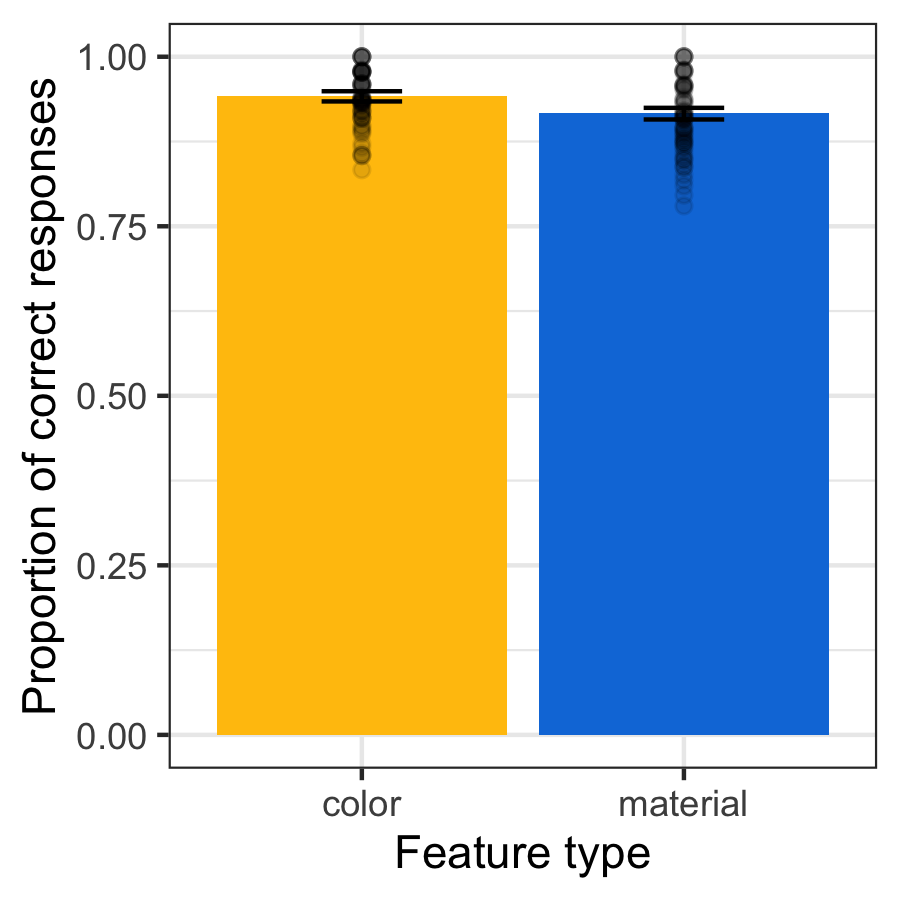
\includegraphics[width=\textwidth]{plots/exp1_proportion.png}
\caption{Proportion of correct responses}
\label{fig:exp1_a}
\end{subfigure} \hspace{9mm}
\begin{subfigure}{.4 \textwidth}
\centering
\includegraphics[width=\textwidth]{plots/exp1_rt.png}
\caption{Response times of correct responses}
\label{fig:exp1_b}
\end{subfigure}
\caption{Response patterns to color and material adjectives in the norming experiment}
\label{fig:exp1}
\end{figure}   

To categorize the image-word pairs in this way, we first grouped them in multiple different ways, always grouping the top 15 image-word combinations in the high-difficulty group and the bottom 15 image-word combinations in the low-difficulty group. First, we grouped pairs by response times, regardless of response correctness and match between the adjective and image. Then we grouped the pairs by response times of correct responses, and then by response times of correct responses to matching features and separately for not-matching features. We also grouped pairs by error rates in three different ways. Finally, we looked at the overlap between these groups and grouped the 8 image-material adjective pairs with the highest error rate and response times into a \textit{high difficulty} group, and the 8 image-color adjective pairs with the lowest error rate and response times into a \textit{low difficulty group}.

\section{Experiment 2: Production of referring expressions} 

The goal of Exp. 2 was to elicit production probabilities of redundantly mentioning color and material adjectives for the high- and low-difficulty items normed in Exp. 1. In a free production interactive reference game we tested whether adjectives that denote more perceptually difficult properties are less frequently produced redundantly.\footnote{Procedure, materials, analysis and exclusions were preregistered at \href {https://osf.io/57c6u}{https://osf.io/57c6u}.}

\subsection{Participants} 

We recruited 100 participants through Amazon Mechanical Turk and randomly paired them into speaker-listener dyads to play a real time communication game (50 pairs) (\citealt{Hawkins2015}). We excluded games where participants reported a native language different from English.

\subsection{Procedure} 

On each trial, participants saw a display with 4 images and chat box. Both the speaker and the listener saw the same images in different positions. One of the images was designated as the target image, and marked by a green border in the speaker's display. The speaker's task was to describe this target image to the listener using the chat box to send messages. The listener's task was to guess the target image by clicking. After the listener made a selection, both participants received feedback about whether the target image was selected and advanced to the next trial. 

\begin{figure}[ht]
   \centering
   \begin{minipage}[t]{0.48\linewidth}
   \centering
   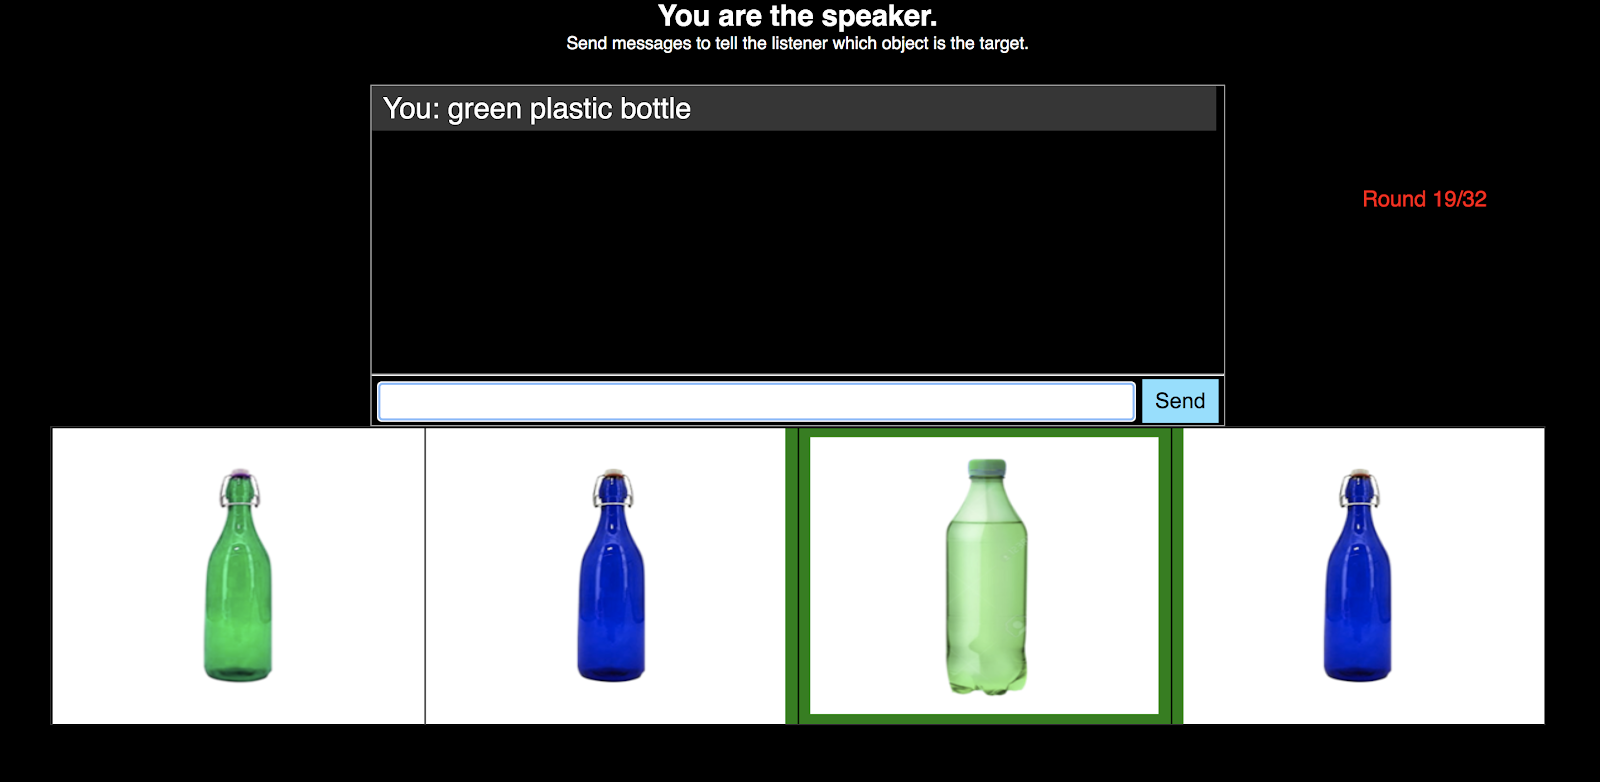
\includegraphics[width=\textwidth, frame]{img/exp2_trial.png}
   \captionof{figure}{Example display from Exp. 2: speaker's perspective on a \textit{low-difficulty (color redundant)} trial}
   \label{fig:exp2_trial}
   \end{minipage}\hfill%
   \begin{minipage}[t]{0.48\linewidth}
   \centering
   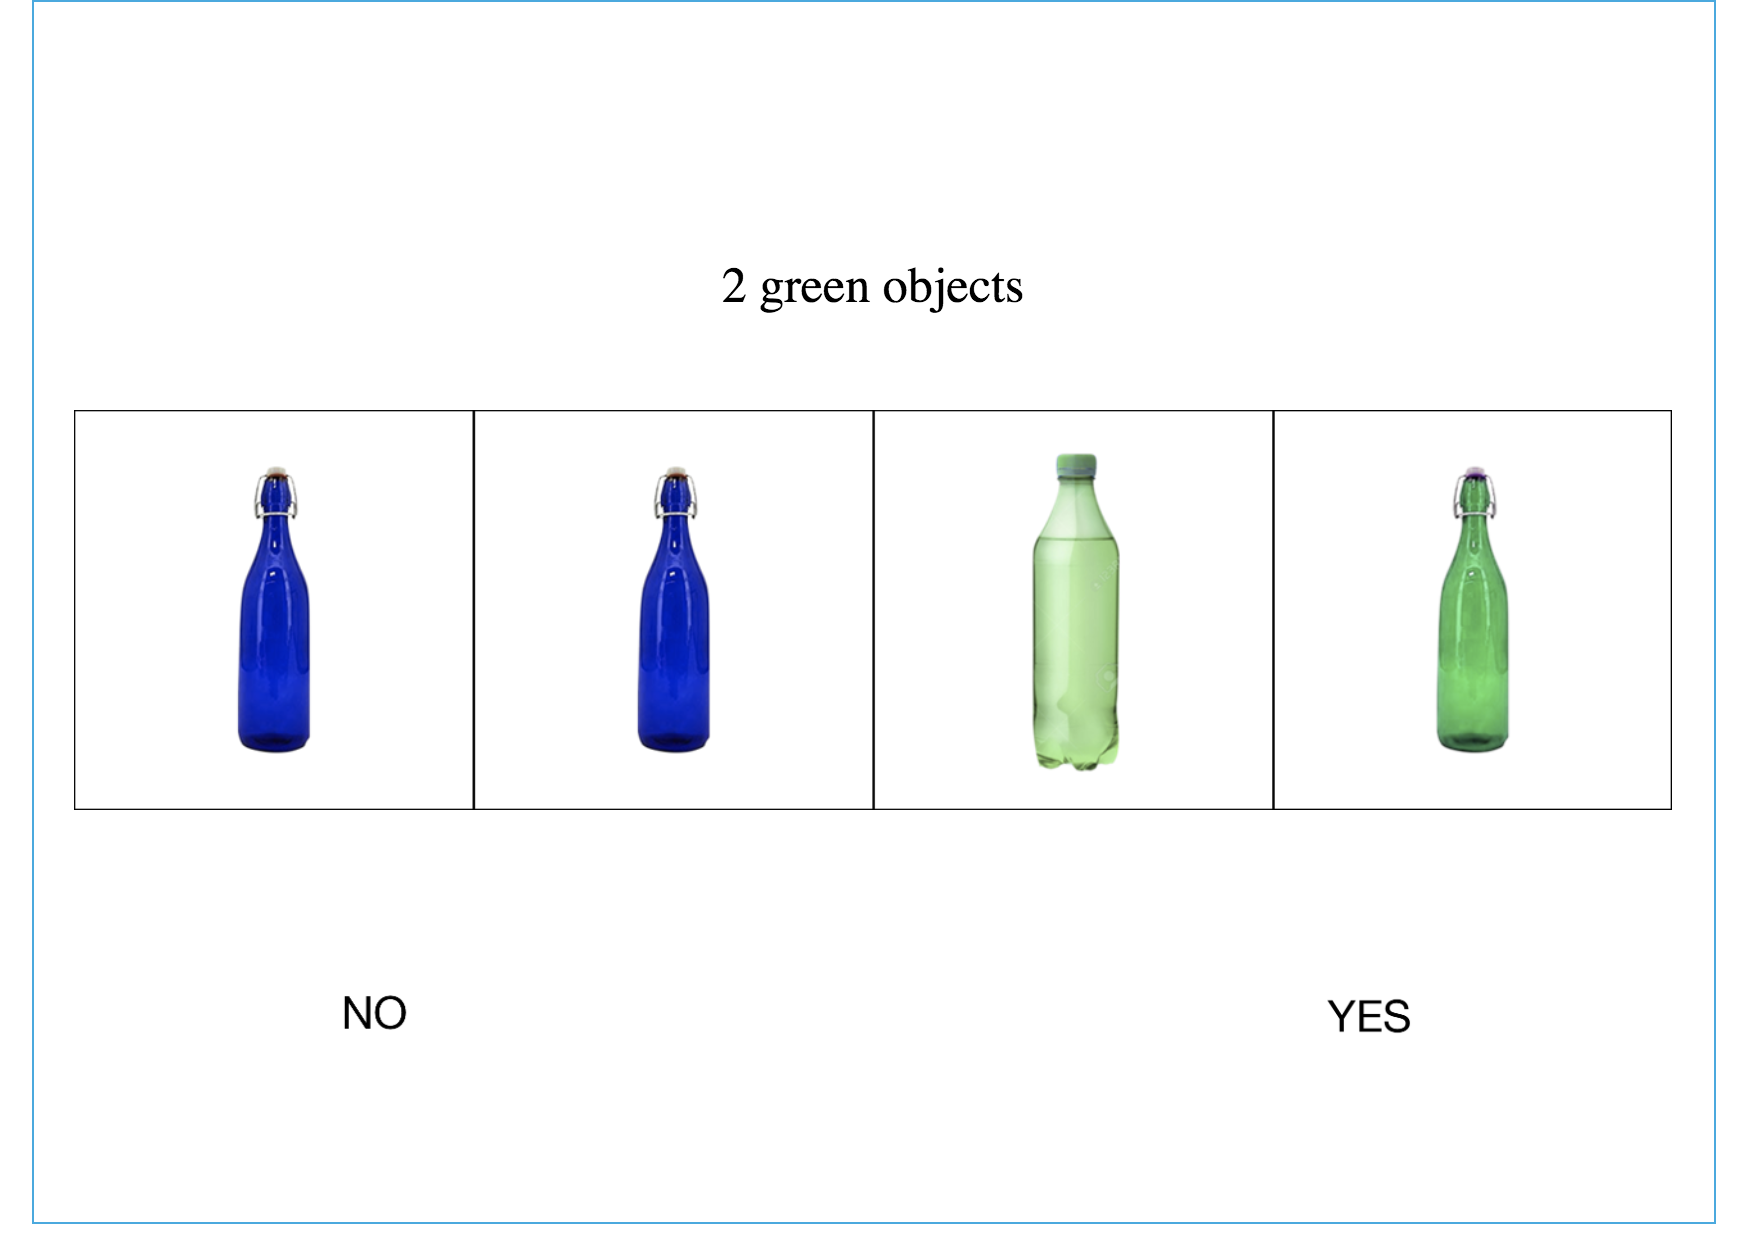
\includegraphics[width=\textwidth, frame]{img/exp3_trial.png}
   \captionof{figure}{Example display from Exp. 3: color trial with correct number}
   \label{fig:exp3_trial}
   \end{minipage}
\end{figure}

Participants completed 32 trials. Of these, half were critical trials and half were filler trials. On critical trials (Figure~\ref{fig:exp2_trial}), the 4 images were of the same object and either \textit{color} or \textit{material} was redundant for distinguishing the target. One of the images, the competitor, always shared the redundant feature with the target and the two distractors shared the sufficient feature with the competitor. On 8 high-difficulty trials, mentioning the material was redundant; on 8 low-difficulty trials, color was redundant. On filler trials, the 4 images were of different objects and both color and material mention were redundant for unique reference. Filler items were of 4 different types: the competitor either shared the color, material, both or none of the features with the target. 

\subsection{Results}

To explore the use of redundant adjectives, we first classified the produced utterances as 'color-and-material' (redundant), 'only-color' or 'only-material'. Proportion of redundant "color and material" utterances and non-redundant utterances are shown in Figure~\ref{fig:exp2_proportion}. We conducted a mixed effects logistic regression predicting redundant adjective use from fixed effects of redundant property, with random by-subject and by-item intercepts and slopes for redundant property. There was a main effect of redundant property, such that speakers were more likely to redundantly mention color than material ($\beta$= 2.32, $SE$=0.64, $p$$<$.0001), replicating the previously observed asymmetry between overmodification with color and material adjectives on a new set of items. Our analysis of the responses to filler trials showed that the preference to mention color transferred to trials in which neither color nor material mention was required for unique reference. 

In a second step, we manually checked for the use of modifiers other than the color and material adjectives. We found that on 39\% of all utterances, participants used a different kind of modifier to reference the target. These modifiers included shape (\textit{rectangular table}), size (\textit{long table}), shade (\textit{dark blue plate}) and type (\textit{solo cup}) modifiers. The full data pattern with color, material and other modifiers revealed that when material was the redundant feature, participants mentioned only the color, and when color was the redundant feature, they either produced color-and-material utterances or overmodified with color and used a modifier denoting a property other than color or material. 

Given the norms from Exp. 1, these results suggest that the more difficult it is to judge whether an object has a feature, the less likely speakers are to redundantly mention that feature, providing initial support for the perceptual difficulty hypothesis. However, these results do not reflect perceptual difficulty differences beyond the property type. Because the difference between response times and error rates for the two properties wasn't large enough, we weren't able to detect perceptual difficulty differences within property type. In order to get more power and replicate this effect with a different dependent measure of perceptual difficulty, we ran a third experiment.

\begin{figure}[ht]
\centering
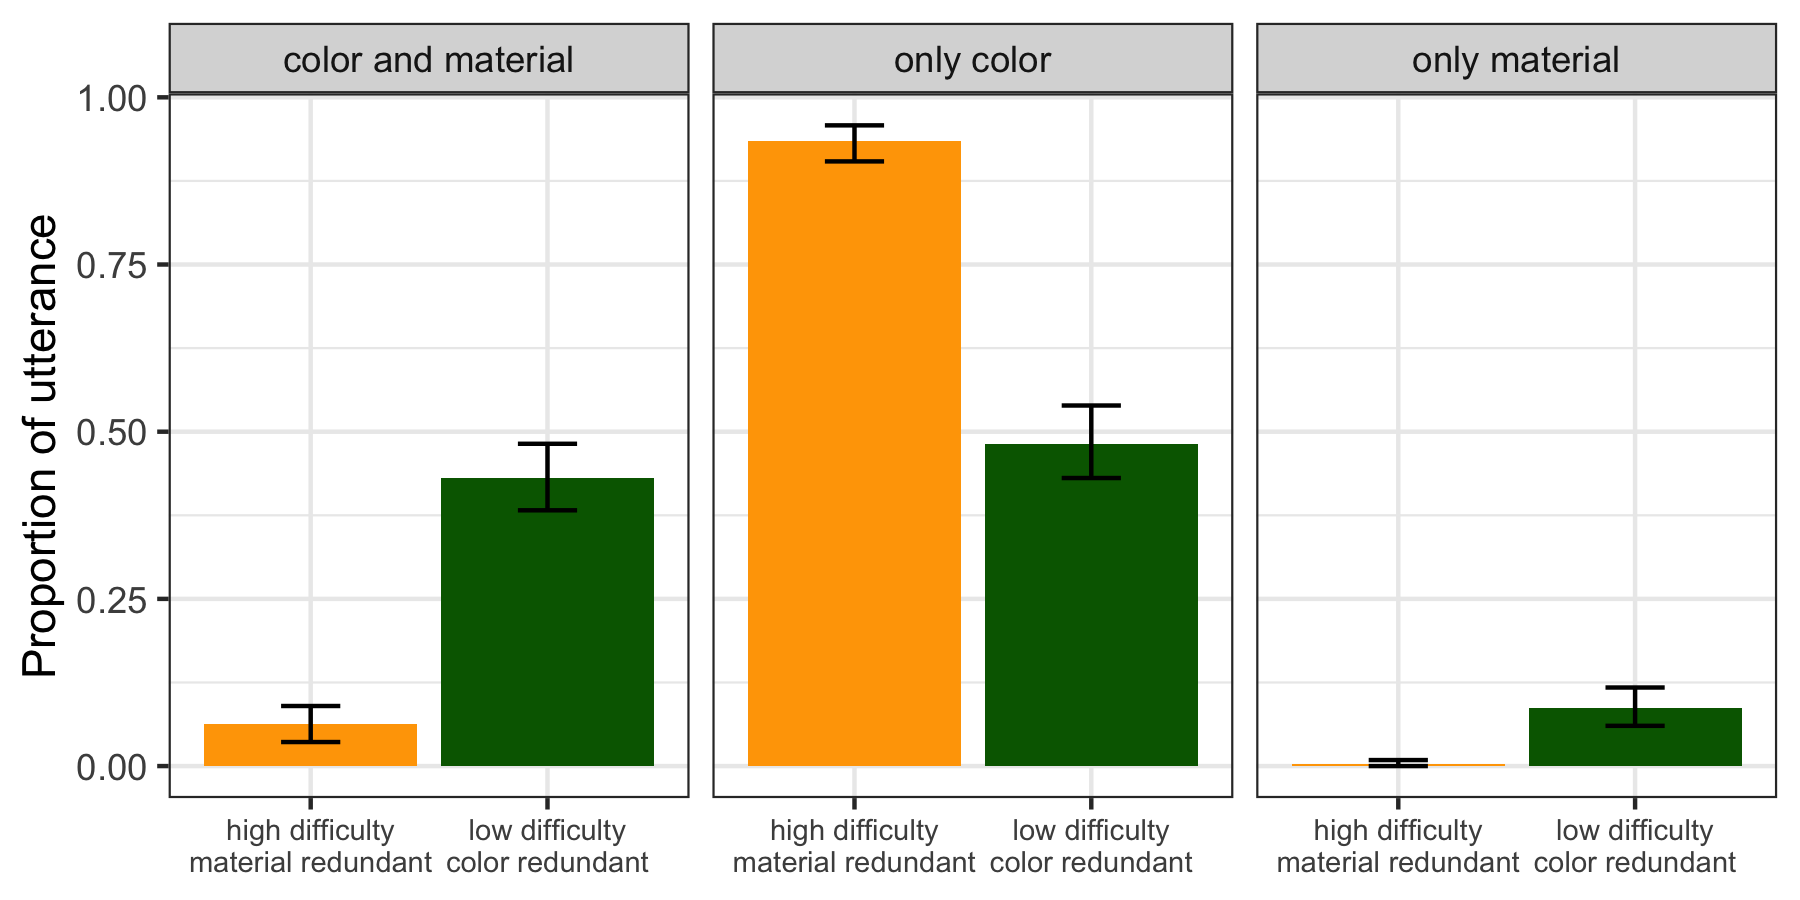
\includegraphics[width=.8\textwidth]{plots/exp2_proportion.png}
\caption{Proportion of redundant "color and material" utterances vs non-redundant utterances in high and low difficulty trials}
\label{fig:exp2_proportion}
\end{figure}

\section{Experiment 3: Perceptual difficulty in context} 

The goal of Exp. 3 was to get a more nuanced measure of perceptual difficulty that takes contextual factors into account and allows to test the effect of perceptual difficulty beyond property type.

\subsection{Participants} 

We recruited 400 participants through Prolific. We excluded participants with accuracy lower than 75\% (n=24) and responses that were too slow (2.5 standard deviations away from the mean response time) (217 responses).

\subsection{Procedure} 

Exp. 3 was identical to Exp. 1 but instead of seeing the images in isolation, participants saw the displays from the production experiment. These displays appeared with short descriptions that were of the form "X [adjective] objects" and included a number and either a color or material adjective (see Fig.~\ref{fig:exp3_trial}). On half of the trials, the statement was correct and on the other half, it was incorrect. The use of color and material adjectives was also balanced. We collected 100 judgements for each feature in the display, for all the different displays.

\subsection{Results} 

First, we analyzed the mean response times to the two property types to address the first question of interest, are properties denoted by material adjectives more perceptually difficult than ones denoted by color adjectives? To this end, we ran a mixed effects linear regression model predicting log-transformed response time from fixed effects of redundant property with random by-participant an by-item intercepts and slopes for redundant property. We found that responses to color adjectives were faster than the responses to material adjectives ($\beta$= 0.24, $SE$=0.018, t=-59.62, $p$$<$.0001), replicating the results of Exp. 1 (see Figure~\ref{fig:exp3}). 

To address the more theoretically interesting question of interest, namely whether perceptual difficulty modulates redundancy within property type, we first analyzed the absolute response times to redundant and sufficient properties of target items of Exp. 2. In order to identify the individual contribution of trial type and mean response time (to redundant adjective) on redundant adjective use, we first performed a residualization step. Since property type is a strong predictor of response time, we regressed the response times against property type using a simple linear model predicting log-transformed response time from trial type ($\beta$= -0.26, $SE$=0.004, t=-71.24, $p$$<$.0001). We then used the residuals of this model as the predictor in a mixed effects logistic regression predicting redundant adjective use. In this analysis, we replicated the effect of trial type on response time ($\beta$= 7.43, $SE$=2.27, $p$$<$.001) but found neither a main effect of response time ($\beta$= -11.3, $SE$=16.41, $p$$=$.49) or interaction between response time and trial type ($\beta$= 13.57, $SE$=31.87, $p$$=$.67) on redundant adjective use. 

To further test the strong version of the perceptual difficulty hypothesis, we used another measure of perceptual difficulty: the relative perceptual difficulty of the sufficient property compared to the redundant property. We computed the log ratio of mean response time to sufficient property to mean response time to redundant property and performed the same residualization step described above. We found no effect of response time beyond trial type ($\beta$= 7.71, $SE$=1.73, $p$$<$.001)).

\begin{figure}[ht]
   \centering
   \begin{subfigure}{.4\textwidth}
   \centering
   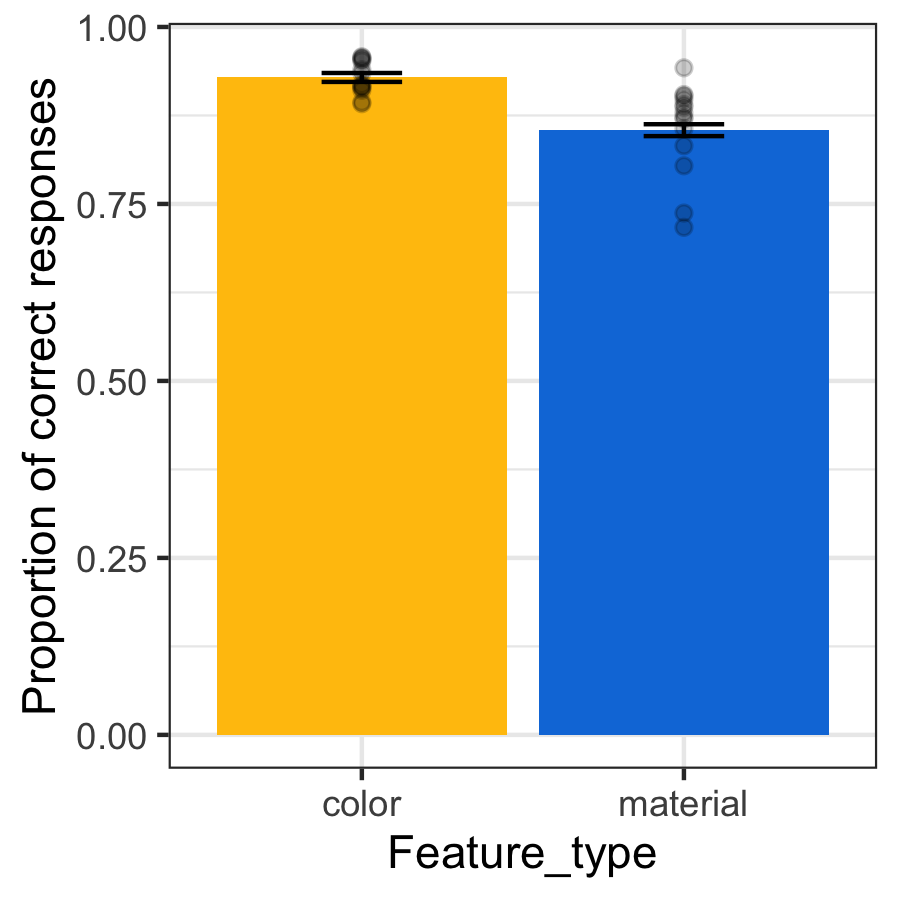
\includegraphics[width=\textwidth]{plots/exp3_proportion.png}
   \caption{Proportion of correct responses}
   \label{fig:exp3_a}
   \end{subfigure} \hspace{9mm}
   \begin{subfigure}{.4 \textwidth}
   \centering
   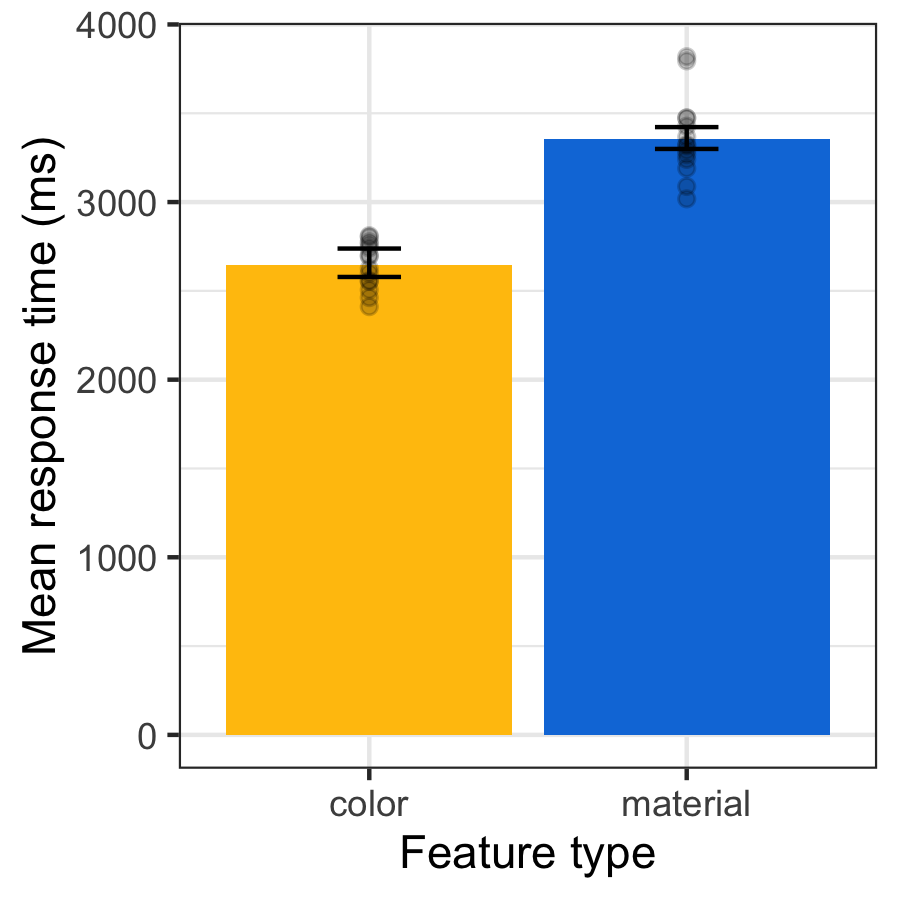
\includegraphics[width=\textwidth]{plots/exp3_rt.png}
   \caption{Response times of correct responses}
   \label{fig:exp3_b}
   \end{subfigure}
   \caption{Response patterns to color and material adjectives in Exp. 3}
   \label{fig:exp3}
\end{figure}   

\section{General discussion} 

We tested the role of perceptual difficulty in explaining the asymmetry in overmodification patterns with color and material adjectives. We predicted that the difference in perceptual difficulty of establishing whether objects are of a particular color or material could explain the asymmetry in the redundant use of color and material adjectives. This prediction is in line with recent work by \citet{RubioEtAl2019} that shows the role of perceptual factors and more specifically, the relative visual saliency of properties denoted by adjectives, in derivation of contrastive inferences.

There are two versions of the perceptual difficulty hypothesis. The work thus far provides evidence for the weak version of this hypothesis, that the propensity to redundantly use color and material adjectives may be driven by the asymmetry in the perceptual difficulty involved in establishing whether or not a particular object is of a particular color or material. Exp. 1 and Exp. 3 both provide support for this hypothesis, since in both experiments color adjectives generally resulted in lower error rates and lower response times than material adjectives. Under the strong version of the hypothesis, perceptual difficulty should modulate redundancy within property type such that for items where establishing the property is more difficult, we should see gradient effects on redundancy. The analysis of the data set we collected so far doesn't provide evidence for the effect of perceptual difficulty beyond property type. 

One avenue of future work is to more explicitly test the strong version of the hypothesis. The items we selected were structured such that there wasn't too much within-category variability, material being more difficult to asses than color categorically. A stronger test would specifically select for bigger within-category perceptual difficulty variability.

Finally, the effects we found are consistent with the efficiency account of redundant adjective use and provide preliminary evidence that the noise term in \citet{DegenEtAl2020}'s computational model of referring expression production might be a function of the perceptual difficulty of properties adjectives denote. Formalizing noisy semantics and informativeness in this way also allows us to be neutral in regards to whether overmodification is a speaker-internal or listener-oriented process (\citealt{Arnold2008}). While some researchers argue that overmodification helps the speaker because the redundant attributes are more easily produced (\citealt{DaviesKatsos2013, KoolenEtAl2013}, others argue that it helps the listener by making it easier to identify the target (\citealt{FussellKraus1989a, ArtsEtAl2011,RubioFernandez2016}). Our task doesn't allow us to adjudicate between these two views. We provide evidence for the speaker internal pressure for redundantly mentioning the less perceptually difficult feature type, but remain agnostic with regards to how this aids listeners in target identification.

% optional: density plots for adjectives tested in each experiment (can format this better)
% \begin{figure}[ht]
%    \centering
%    \begin{subfigure}{.3\textwidth}
%    \centering
%    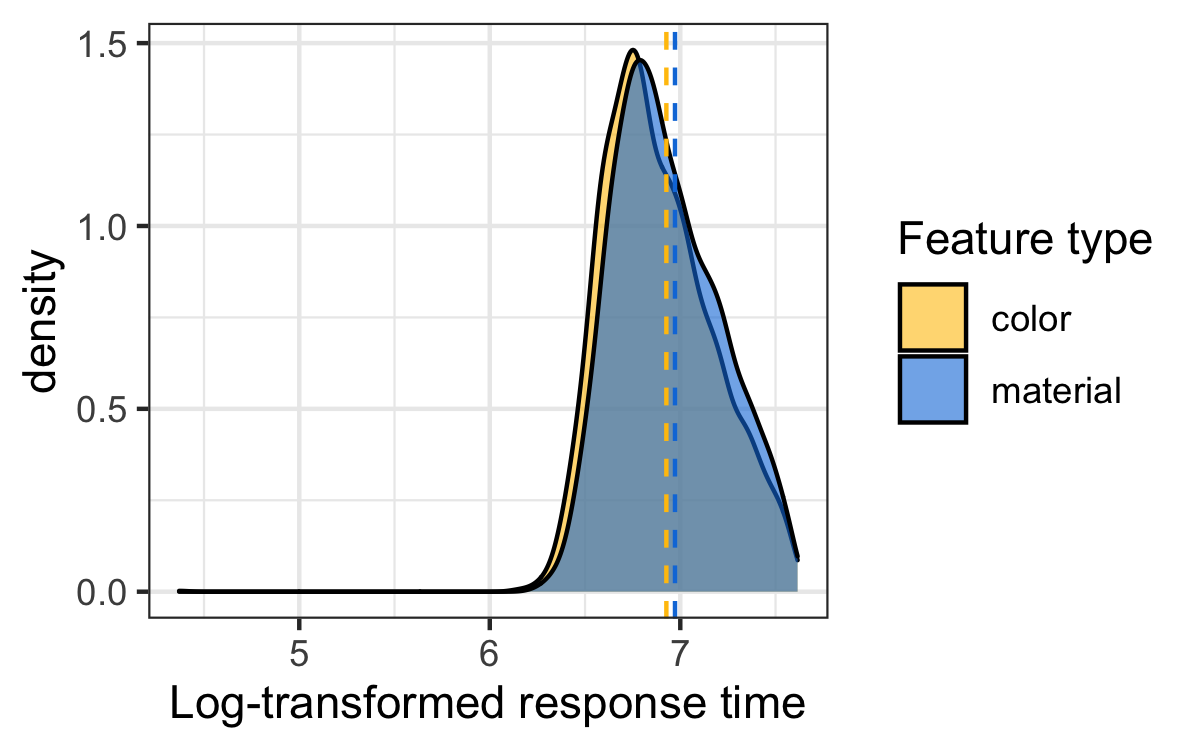
\includegraphics[width=\textwidth]{plots/exp1_density_logRT.png}
%    \caption{Exp. 1}
%    \label{fig:density_1}
%    \end{subfigure} \hspace{9mm}
%    \begin{subfigure}{.3\textwidth}
%    \centering
%    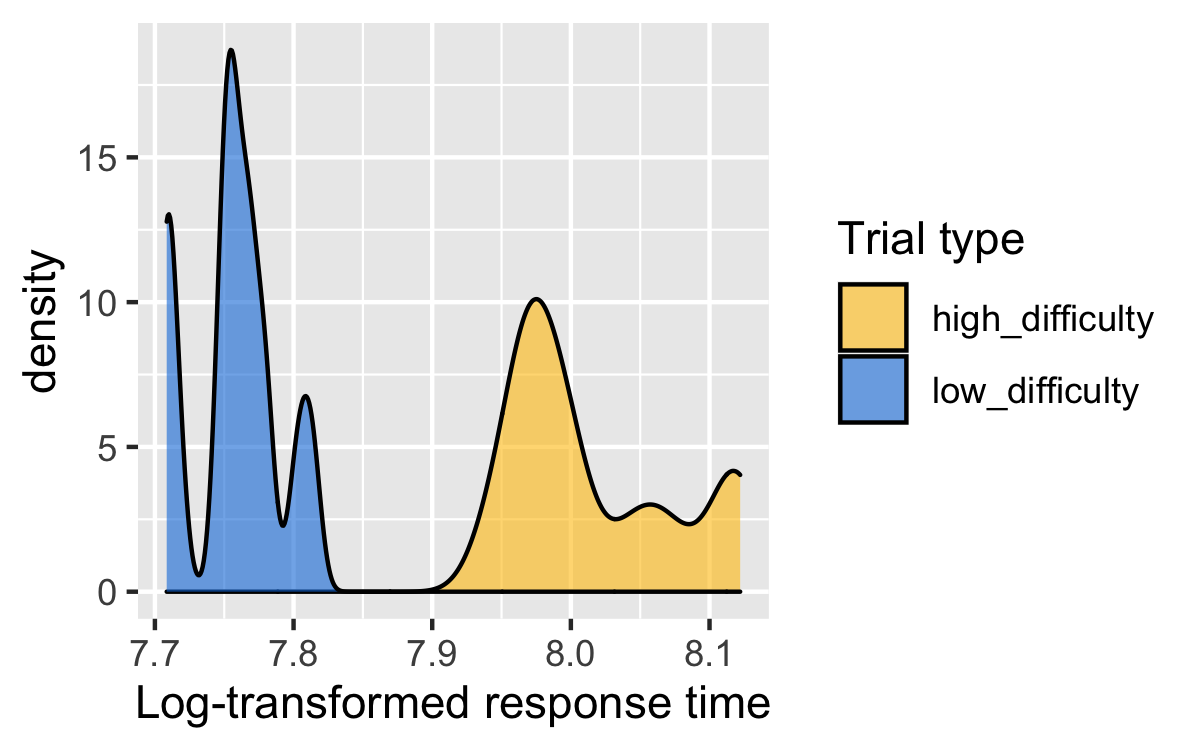
\includegraphics[width=\textwidth]{plots/exp23_density_logRT.png}
%    \caption{Exp. 2}
%    \label{fig:density_2}
%    \end{subfigure}
%    \begin{subfigure}{.3\textwidth}
%    \centering
%    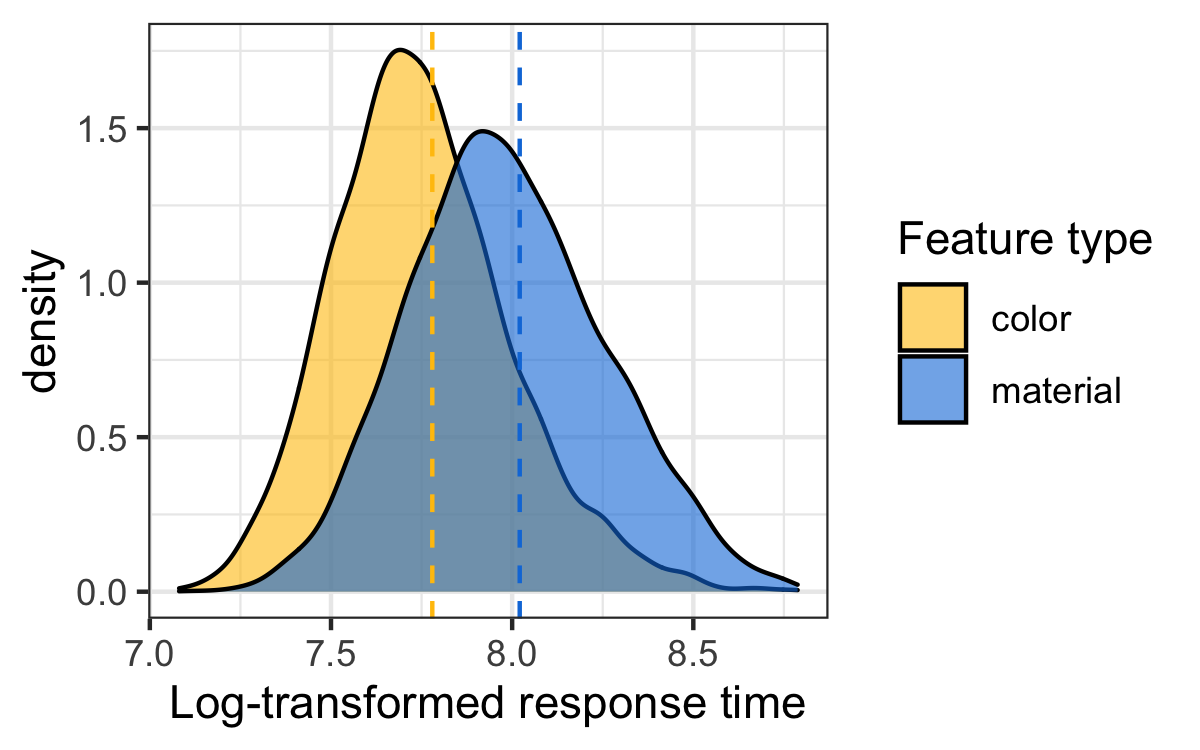
\includegraphics[width=\textwidth]{plots/exp3_density_logRT.png}
%    \caption{Exp. 3}
%    \label{fig:density_3}
%    \end{subfigure}
%    \caption{Distribution of log-transformed response times to adjectives tested in different experiments}
%    \label{fig:density}
% \end{figure}  


% \section{Citations and references} Use author-date notation for in-text citations, for example: ... as noted recently by Jameson (2012) and Mateus (2014), drawing on insights from various other researchers (e.g., Nelson 1986:223–28, Martin 2003, Wellington \& Johnson 2016), there have been numerous technological advances in the procedures used to publish research articles online. Include URLs or DOIs with active hyperlinks in citations. The \textit{Semantics and Pragmatics} stylesheet \href{https://raw.githubusercontent.com/semprag/tex/master/sp.bst}{sp.bst} meets the LSA formatting requirements for the list of references, and so may be used. See \href{http://info.semprag.org}{info.semprag.org}. 
% ------------ references --------------------------------------------------------------------------------------
\setlength{\bibsep}{0pt plus 0.3ex}
\setlength{\bibhang}{0.3in}			% hanging indent for references must be 0.3in
\titleformat{\section}{\normalfont\bfseries}{\thesection}{.5em}{}		
% references section not supposed to be followed by a period

\bibliographystyle{sp.bst}	
% \bibliographystyle{apacite}

% S\&P bibliography style
% S\&P, an LSA publication, meets the LSA guidelines. 
% See: http://info.semprag.org 
% and get the bst at: https://raw.githubusercontent.com/semprag/tex/master/sp.bst 
% If using the sp.bst, the following command turns your DOIs into links
\newcommand{\doi}[1]{\href{http://dx.doi.org/#1}{http://dx.doi.org/#1}}	%modified from sp.cls

\bibliography{pd-references}			% your bib file

\end{document}